\chapter{Improving Automated Testing}
For this sprint we have chosen to work on three user stories that should improve automated testing. We work on making automated monkey testing work, making a test that automatically checks if apps are compatible and provide code coverage metrics for the other groups.

\section{Monkey Testing}
During sprint 1 we encountered some difficulties related to monkey testing. In order to monkey test we need to install the apps on an Android device, but we did not have these easily available. Having signed APKs so that they can be uploaded to Google Play, as detailed in \chapterref{sec:upload_google_play}, we can move these APKs to an FTP server so that the monkey tests can always access the newest release version. Each job on Jenkins automatically moves the signed APK to \mono{/srv/ftp/}.

To install a specific app to an Android device, we use the script seen in \listingref{lst:find_newest_apk}, parsing to it the application id of the app. All APKs containing the given application id is then found. This result is piped to \mono{sed 's|.*b||' |'s|\_release\_aligned.apk||' } that removes everything but the build number of the files. \mono{awk '\$0>x\{x=\$0\};END\{print x\}'} then finds the maximum build number. Finally the newest APK for the given application id is found.

\begin{lstlisting}[language=bash,showstringspaces=false,caption=Script that finds the newest build number for a particular application id,label=lst:find_newest_apk]
NEWEST_BUILD="$(find /srv/ftp/newest_apks/ -name "$1*release_aligned.apk" | sed 's|.*b||' | sed 's|_release_aligned.apk||' | awk '$0>x{x=$0};END{print x}')"
find /srv/ftp/newest_apks/ -name "$1*b${NEWEST_BUILD}_release_aligned.apk"
\end{lstlisting}

When the app has been installed on the device, we run a monkey test on it using the Jenkins plugin. Starting a monkey test will launch the app. This poses problems for the majority of the Giraf apps, as they require extra information when starting, such as user information. If the apps are not given this information at launch they will crash. This means that all monkey tests report failure. The only app that require no extra information is the launcher. However, as the launcher uses the first 5--10 minutes downloading pictograms, the monkey test only presses on a loading screen.

The \mono{monkey} command does not support sending extra information when starting apps. We did not anticipate this obstacle and did therefore not manage to implement monkey testing for apps fully.

\section{App Installation Test Case}
To ensure that all apps of the multi-project are compatible a test on Jenkins is run nightly that installs all apps on a single device. At the end of sprint 1 the GUI groups had issues installing a combination of apps on a single device --- this test case should avoid such an issue in the future.

To do this we find the newest version of all available APKs on the server. These APKs are the same that are uploaded to Google Play. The script seen in \listingref{lst:find_all_newest_apks} finds the application id for each available app by finding all files in the directory containing APKs. It then pipes these files to \mono{sed 's|.*/||'} which removes the path of the file. This is then piped to \mono{sed 's|\_v.*||'} that removes everything following the package id. The output of that is then sorted and all duplicates are removed using \mono{sort | uniq}. The sort is necessary as \mono{uniq} only removes duplicate lines that are adjacent. 

The application names are then send to \mono{find\_newest\_apk.sh}, as seen previously in \listingref{lst:find_newest_apk}.

\begin{lstlisting}[language=bash,showstringspaces=false,caption=Script that finds the newest available APK for all apps,label=lst:find_all_newest_apks]
PACKAGE_NAMES="$(find /srv/ftp/newest_apks/ -name "*release_aligned.apk" | sed 's|.*/||' | sed 's|_v.*||' | sort | uniq)"


for p in $PACKAGE_NAMES
do
    /srv/scripts/find_newest_apk.sh $p
done
\end{lstlisting}

When the newest available APK for each app has been found, they are installed on an Android device. Line 3 tries to install an APK and stores the output in \mono{INSTALL\_OUTPUT}. The output is stored, as \mono{adb install} gives an error code of 0, even if it fails. We therefore have to read the output to check if an error occurred so that Jenkins will report the job as a failure. This is done at line 6 where we check that the output contains the string \mono{success}. The \mono{-i} option makes \mono{grep} case insensitive. At line 9 -- 10 we exit with 1 if the output does not contain \mono{success}.

\begin{lstlisting}[language=bash,showstringspaces=false,caption=Script that installs the given APKs to an Android device,label=lst:install_apks_on_android_device]
for a in $@
do
    INSTALL_OUTPUT="$(/srv/android-sdk-linux//platform-tools/adb install $a)"
    echo $INSTALL_OUTPUT

    IS_SUCCESS="$(echo "$INSTALL_OUTPUT" | grep -i success)"

    # Check if output message does not contain success, since adb install does not provide exit code != 0 at failure
    if ! [ "$IS_SUCCESS" ]; then
        echo "Error installing $a"
        exit 1
    fi
done
\end{lstlisting}

If the installation of any app fails on the device, the Jenkins job will fail.

\section{Code Coverage Reports}
We have a user story which states that Jenkins should provide code coverage metrics for every project. This user story was generated by a group which was writing test of a database project and wanted a measure of their progress. Their main request is for a percentage of lines of code covered. A tool for code coverage report must at least provide this metric, but other more detailed metrics will also be nice to have. In version 0.10 of the New Android SDK Build System \parencite{new-build-android}, support for the JaCoCo \parencite{jacoco-home} Java Code Coverage Library was included. It meets all of our demands for metrics and is nicely integrated into the Android and Gradle build system. To make JaCoCo generate a report all one needs to do is to add the code shown in \listingref{lst:Jacoco} to the \mono{build.gradle} file of the project.

\begin{gradlecode}[caption=Gradle script for enabling JaCoCo,label=lst:Jacoco]
dependencies {
    mavenCentral()
}
android {
    buildTypes {
        debug {
            testCoverageEnabled true
        }
    }
}
\end{gradlecode}{}

Now we generate code coverage reports for debug builds locally and in Jenkins. We would like to also publish the code coverage results in Jenkins. There exists a Jenkins plugin \parencite{jacoco-jenkins-plugin} for this purpose. This plugin is easy to setup, provides detailed coverage statistics, and an overview with the percentage of lines of code covered. We use this plugin for publishing the code coverage metrics in Jenkins. An example of this can be seen in \figureref{fig:jenkins-overview-coco}

\begin{figure}[htbp]
    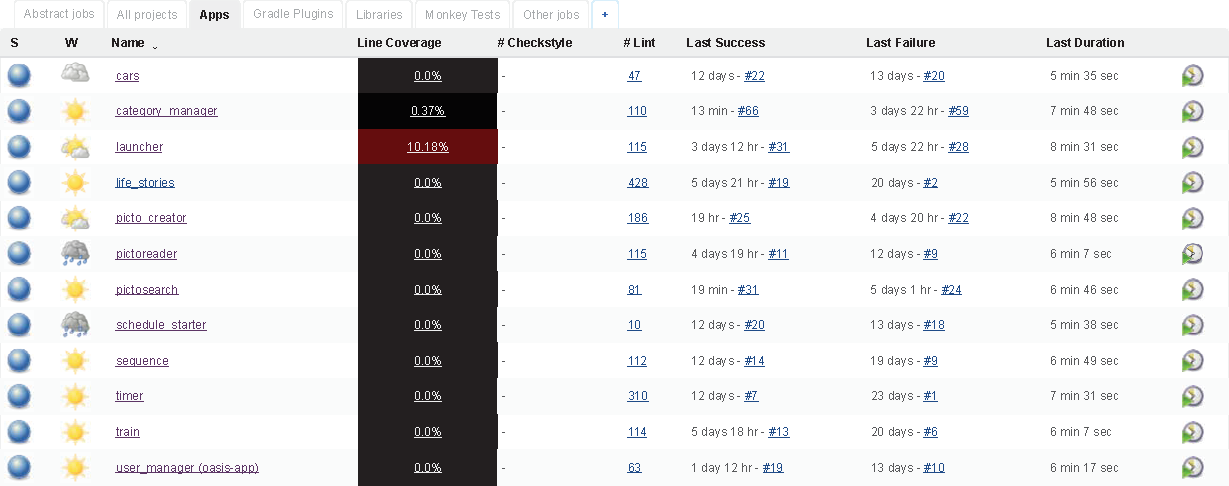
\includegraphics[width=\textwidth]{graphics/jenkins-overview-coco.pdf}
    \caption{Screenshot of a section of the build overview screen which shows the code coverage column}
    \label{fig:jenkins-overview-coco}
\end{figure}